% Created 2018-04-09 lun 18:27
% Intended LaTeX compiler: pdflatex
\documentclass[xcolor={usenames,svgnames,dvipsnames}]{beamer}
\usepackage[utf8]{inputenc}
\usepackage[T1]{fontenc}
\usepackage{graphicx}
\usepackage{grffile}
\usepackage{longtable}
\usepackage{wrapfig}
\usepackage{rotating}
\usepackage[normalem]{ulem}
\usepackage{amsmath}
\usepackage{textcomp}
\usepackage{amssymb}
\usepackage{capt-of}
\usepackage{hyperref}
\usepackage{color}
\usepackage{listings}
\usepackage{mathpazo}
\usepackage{gensymb}
\usepackage{amsmath}
\usepackage{chemarr}%flechas para reacciones químicas (SFER.tex)
\bibliographystyle{plain}
\AtBeginSubsection[]{\begin{frame}[plain]\tableofcontents[currentsubsection,sectionstyle=show/shaded,subsectionstyle=show/shaded/hide]\end{frame}}
\AtBeginSection[]{\begin{frame}[plain]\tableofcontents[currentsection,hideallsubsections]\end{frame}}
\usepackage[emulate=units]{siunitx}
\sisetup{fraction=nice, decimalsymbol=comma, retain-unity-mantissa = false}
\newunit{\wattpeak}{Wp}
\newunit{\watthour}{Wh}
\newunit{\amperehour}{Ah}
\hypersetup{colorlinks=true, linkcolor=Blue, urlcolor=Blue}
\renewcommand{\thefootnote}{\fnsymbol{footnote}}
\beamertemplatenavigationsymbolsempty
\setbeamertemplate{footline}[frame number]
\setbeamercolor{alerted text}{fg=blue!50!black} \setbeamerfont{alerted text}{series=\bfseries}
\usetheme[hideothersubsections]{Goettingen}
\usecolortheme{rose}
\usefonttheme{serif}
\author{Oscar Perpiñán Lamigueiro \\ \url{http://oscarperpinan.github.io}}
\date{}
\title{SFCR: Conceptos Generales}
\hypersetup{
 pdfauthor={Oscar Perpiñán Lamigueiro \\ \url{http://oscarperpinan.github.io}},
 pdftitle={SFCR: Conceptos Generales},
 pdfkeywords={},
 pdfsubject={},
 pdfcreator={Emacs 25.2.2 (Org mode 9.1.9)}, 
 pdflang={Spanish}}
\begin{document}

\maketitle

\section{Sistemas Fotovoltaicos de Conexión a Red}
\label{sec:orgfb9050f}

\subsection{Definición}
\label{sec:org6ce806d}

\begin{frame}[label={sec:org144e737}]{Definición de un SFCR}
\begin{block}{}
Un Sistema Fotovoltaico Conectado a la Red (SFCR) es un sistema cuya
función es producir energía eléctrica en condiciones adecuadas para
poder ser inyectada en la red convencional.

\begin{center}
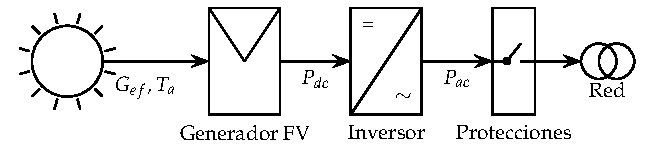
\includegraphics[width=.9\linewidth]{../figs/EsquemaSFCR.pdf}
\end{center}
\end{block}
\end{frame}

\subsection{Mecanismos de Retribución}
\label{sec:orgac98b44}
\begin{frame}[label={sec:orgacf90fa}]{Mecanismos de retribución}
\begin{itemize}
\item La energía producida por este sistema será consumida parcial o totalmente en las cercanías, y la energía sobrante será inyectada en la red para su distribución a otros puntos de consumo.

\item Mecanismos de retribución

\begin{itemize}
\item Prima (\emph{Feed-in tariff})

\item Balance neto (\emph{Net-metering})
\end{itemize}
\end{itemize}
\end{frame}

\begin{frame}[label={sec:orge2c9fc7}]{Retribución con prima}
\begin{itemize}
\item \alert{Ingresos} por la \alert{energía total producida} (independientemente de la que
haya sido consumida en las cercanías del SFCR).

\item El diseño \alert{no necesita considerar un consumo} a satisfacer.

\item \alert{Objetivo}: producción anual del sistema sea la máxima posible sin
tomar en consideración los consumos cercanos.
\end{itemize}
\end{frame}

\begin{frame}[label={sec:org35681ed}]{Balance neto}
\begin{itemize}
\item \alert{Compensa los saldos de energía eléctrica} entre el SFCR y un sistema de consumo asociado.

\item Cuando la producción del SFCR supera al consumo, la red eléctrica absorbe el excedente puntual, generándose derechos de consumo diferido.

\item Estos derechos de consumo se pueden ejercer cuando la producción del SFCR no es suficiente para satisfacer el consumo asociado.

\item El \alert{diseño debe incluir el consumo asociado} como una \emph{variable adicional} que condicionará el tamaño del generador fotovoltaico.
\end{itemize}
\end{frame}


\subsection{SFCR en suelo y en edificación}
\label{sec:org9764daf}
\begin{frame}[label={sec:orgc64209a}]{Características distintivas sobre suelo y en edificación}
\begin{itemize}
\item \alert{Sobre suelo}

\begin{itemize}
\item Sistemas estáticos, con una inclinación y orientación fija

\item Sistemas de seguimiento, que varían la posición del generador a lo
largo del día y año para maximizar la radiación efectiva incidente
\end{itemize}

\item \alert{Sobre edificación}, según el grado de integración

\begin{itemize}
\item General

\item Superposición de módulos: colocación paralela a la envolvente del
edificio

\item Integración arquitectónica: doble función energética y
arquitectónica; sustituyen elementos constructivos convencionales
o son elementos constituyentes de la composición arquitectónica
\end{itemize}
\end{itemize}
\end{frame}


\begin{frame}[label={sec:orgafb6edb}]{SFCR sobre suelo}
\begin{itemize}
\item \alert{Objetivo}: maximizar la producción energética anual del sistema con
el menor coste y la menor ocupación de terreno posibles

\item El diseñador debe decidir el tamaño del generador teniendo en cuenta:

\begin{itemize}
\item Inversión económica (relacionada principalmente con la potencia
del generador)

\item Rendimiento económico deseado (relacionado con la energía
producida por el sistema y, por tanto, con el modo de seguimiento
empleado)

\item Ocupación de terreno (relacionado con el modo de seguimiento
empleado).
\end{itemize}
\end{itemize}
\end{frame}


\begin{frame}[label={sec:org3c8a5a1}]{Estructuras sobre suelo}
\begin{center}
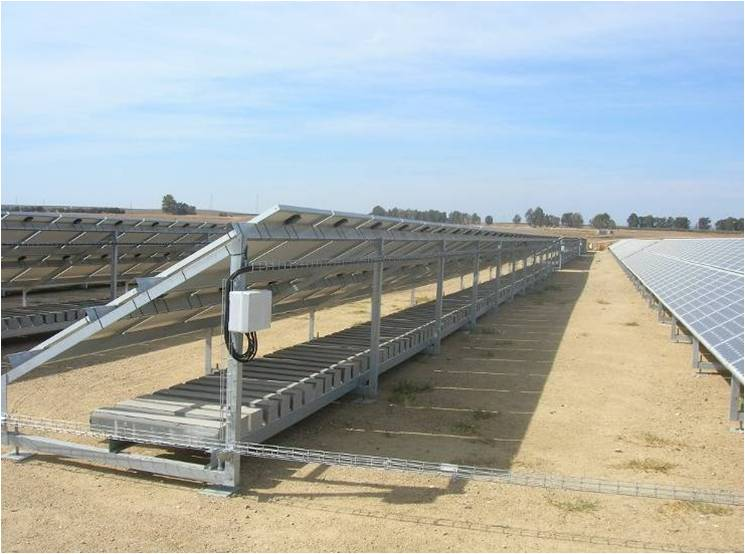
\includegraphics[width=.9\linewidth]{../figs/EstructuraEstaticaSuelo.jpg}
\end{center}
\end{frame}

\begin{frame}[label={sec:orga7166db}]{SFCR sobre suelo: seguimiento}
\begin{itemize}
\item \alert{Fundamento:}

\begin{itemize}
\item Radiación incidente aumenta al seguir al sol

\item Pérdidas por reflexión disminuyen si el apuntamiento al sol mejora
\end{itemize}

\item Las diferentes técnicas de seguimiento son un compromiso entre un
apuntamiento perfecto y sistemas estructurales más económicos y
mejores aprovechamientos del terreno.
\end{itemize}
\end{frame}

\begin{frame}[label={sec:org78a8b12}]{SFCR sobre suelo: seguimiento}
\begin{itemize}
\item \alert{Doble eje}

\begin{itemize}
\item Apuntamiento \guillemotleft{}perfecto\guillemotright{}

\item Mejor productividad, peor ocupación de terreno.
\end{itemize}

\item \alert{Seguimento acimutal}

\begin{itemize}
\item Sacrifica un movimiento (inclinación del generador) para conseguir
sistemas más económicos.
\end{itemize}

\item \alert{Seguimiento horizontal con eje Norte-Sur}

\begin{itemize}
\item Sencillez y estabilidad estructural (el eje es horizontal y
paralelo al terreno, con tantos puntos de apoyo como se consideren
necesarios),

\item Facilidad de motorización,

\item Buen aprovechamiento del terreno.
\end{itemize}
\end{itemize}
\end{frame}


\begin{frame}[label={sec:orgb2d9b7f}]{Seguidor de eje horizontal N-S}
\begin{center}
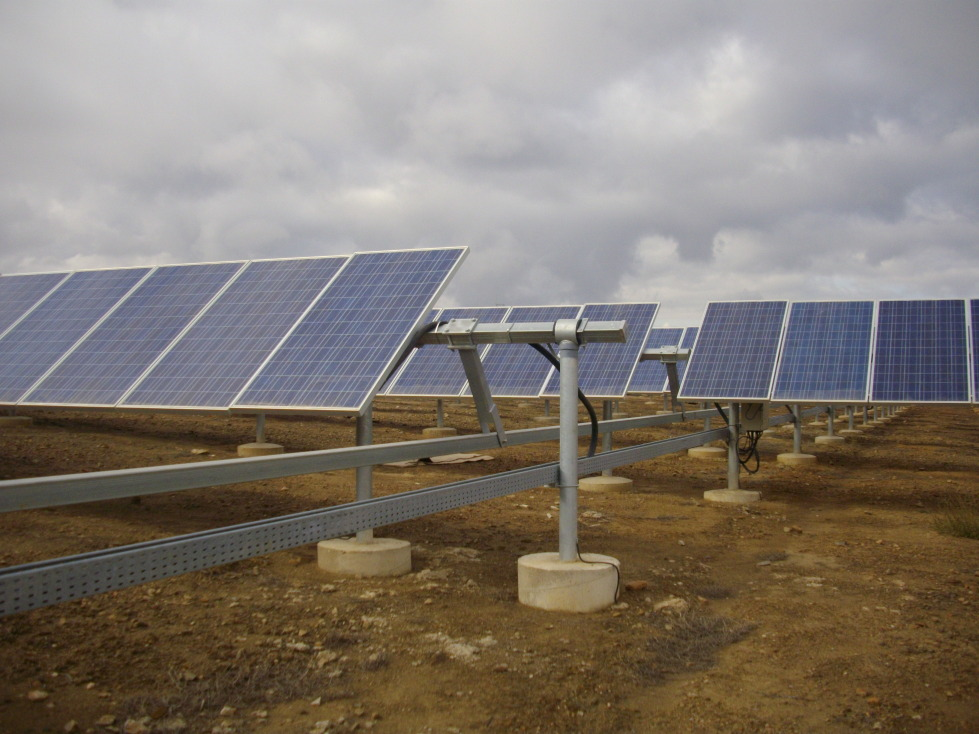
\includegraphics[width=.9\linewidth]{../figs/SeguidorEjeHorizontal.jpg}
\end{center}
\end{frame}


\begin{frame}[label={sec:org883c5cf}]{Seguidor de doble eje}
\begin{center}
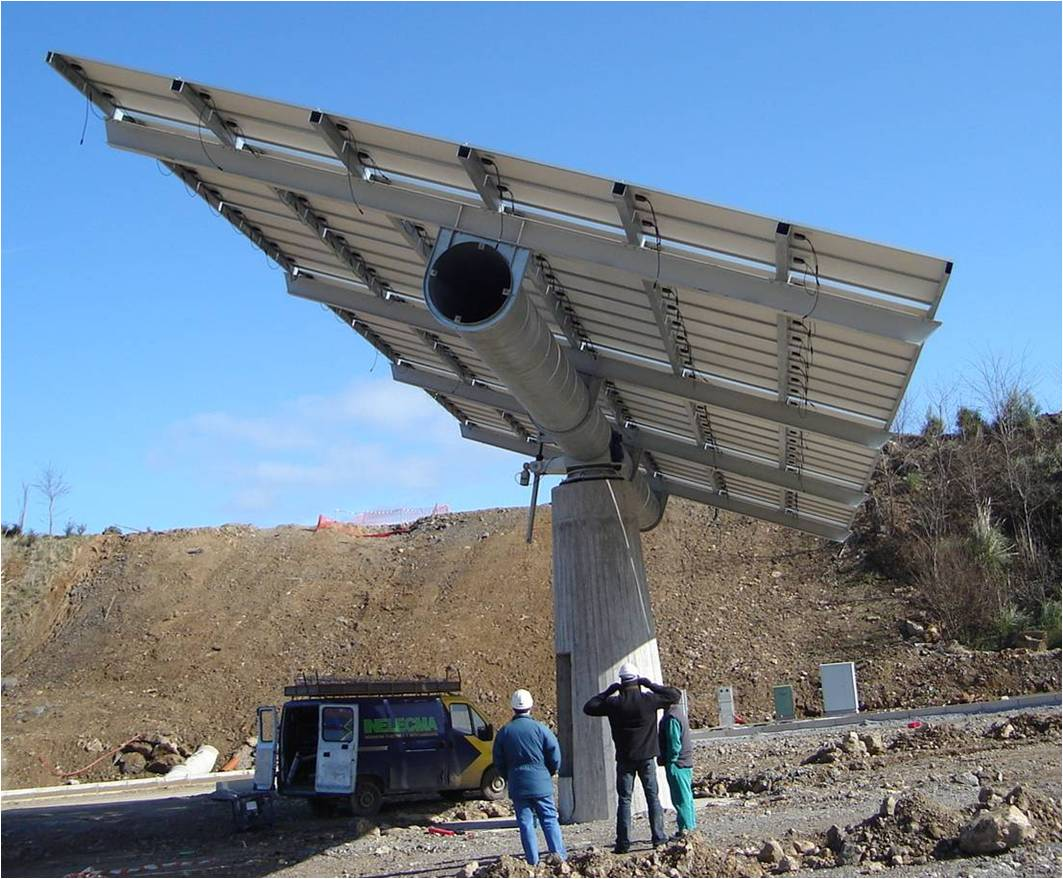
\includegraphics[width=.9\linewidth]{../figs/SeguidorReocin.jpg}
\end{center}
\end{frame}

\begin{frame}[label={sec:org28d2153}]{SFCR en edificación}
\begin{itemize}
\item La integración del sistema fotovoltaico con el edificio exige tener en cuenta muchos factores que condicionan la ubicación y la configuración del generador.

\item El diseñador debe tomar las decisiones oportunas para \alert{aprovechar las sinergias entre edificio y sistema fotovoltaico}, reduciendo las posibles interferencias entre uno y otro.
\end{itemize}
\end{frame}

\begin{frame}[label={sec:org6d0e996}]{Integración arquitectónica}
\begin{itemize}
\item Cubierta Inclinada
\item Cubierta Plana
\item Parasol
\item Fachada Acristalada
\item Muro Cortina
\item Aparcamiento
\item \ldots{}
\end{itemize}

\begin{block}{}
\url{http://www.pvdatabase.org/}
\end{block}
\end{frame}

\begin{frame}[label={sec:org26febb7}]{Cubierta Inclinada}
\begin{center}
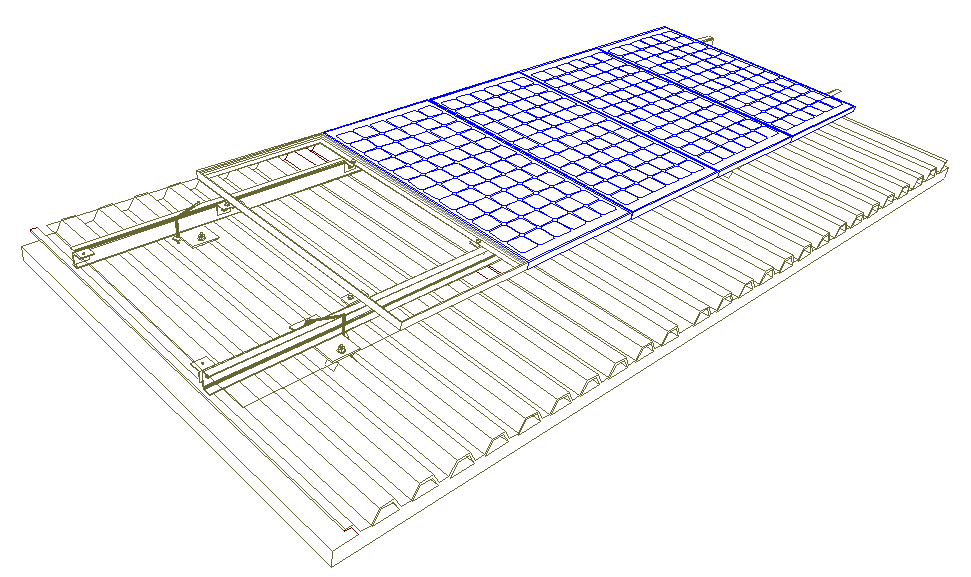
\includegraphics[width=.9\linewidth]{../figs/CubiertaInclinada.png}
\end{center}
\end{frame}

\begin{frame}[label={sec:org582bf95}]{Cubierta Plana}
\begin{center}
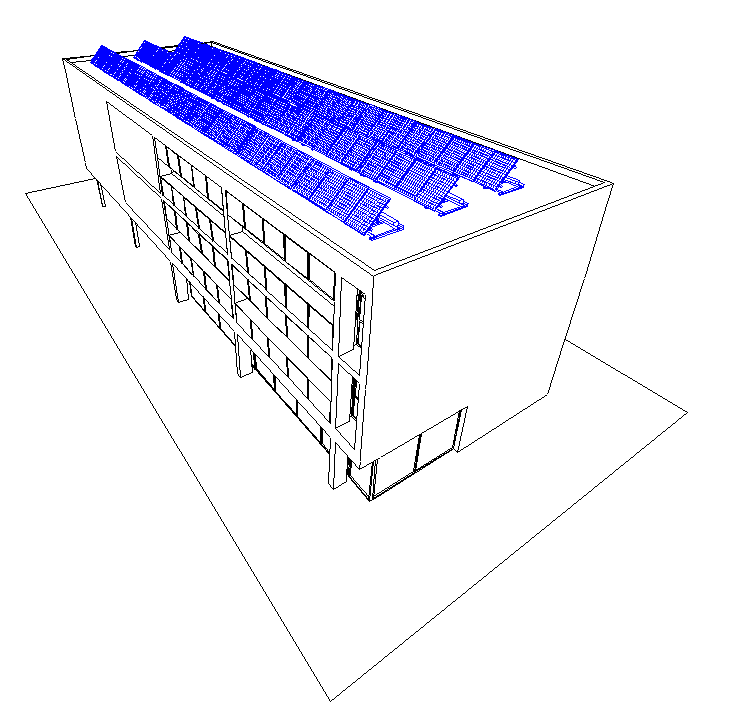
\includegraphics[width=.9\linewidth]{/home/oscar/github/esf/figs/CubiertaPlana.png}
\end{center}
\end{frame}

\begin{frame}[label={sec:orga4c1d15}]{Parasol}
\begin{center}
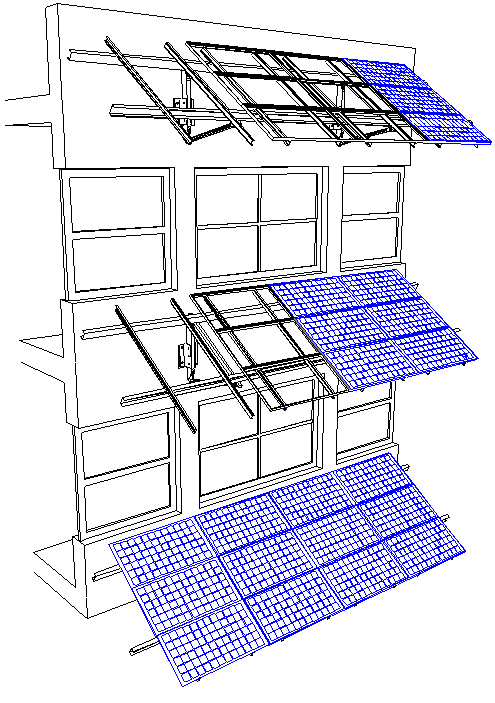
\includegraphics[height=0.9\textheight]{/home/oscar/github/esf/figs/Parasol.png}
\end{center}
\end{frame}

\begin{frame}[label={sec:org63f5ef8}]{Fachada Acristalada}
\begin{center}
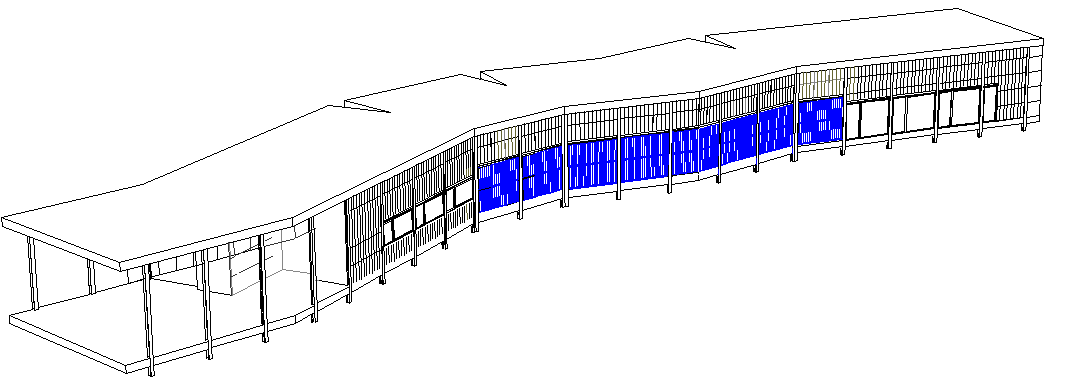
\includegraphics[width=.9\linewidth]{/home/oscar/github/esf/figs/FachadaAcristalada.png}
\end{center}
\end{frame}

\begin{frame}[label={sec:org331f5a4}]{Muro Cortina}
\begin{center}
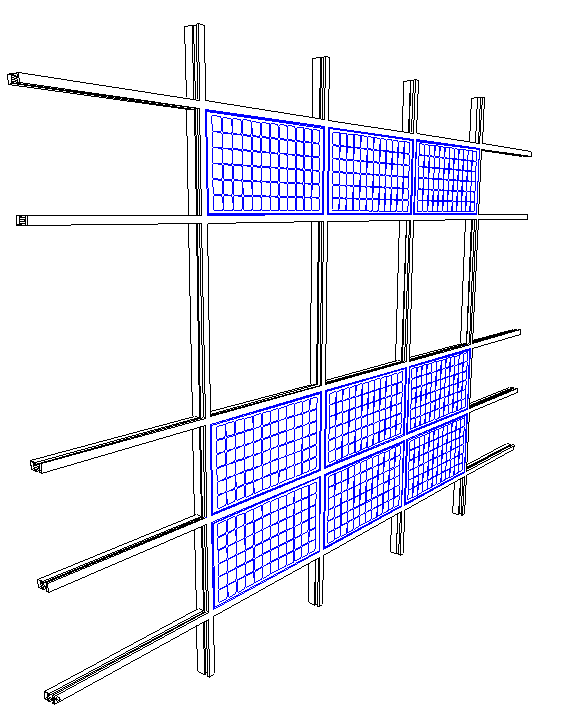
\includegraphics[height=0.9\textheight]{/home/oscar/github/esf/figs/MuroCortina.png}
\end{center}
\end{frame}

\begin{frame}[label={sec:org94630ec}]{Aparcamiento}
\begin{center}
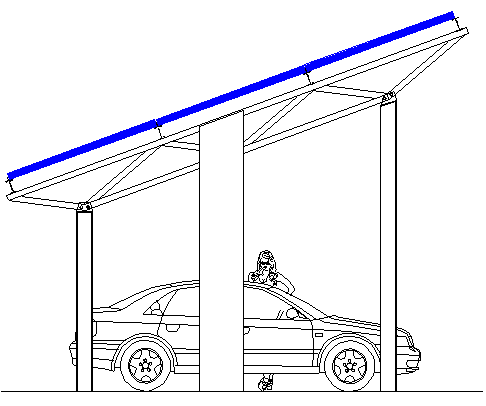
\includegraphics[height=0.8\textheight]{/home/oscar/github/esf/figs/Aparcamiento.png}
\end{center}
\end{frame}


\begin{frame}[label={sec:org0cbcf7e}]{SFCR en edificación: CTE-HE5}
\begin{itemize}
\item El CTE-HTE5 divide España en cinco zonas climáticas de acuerdo al valor medio anual de la radiación global diaria en el plano horizontal.

\item Por ejemplo, toda la cornisa cantábrica está encuadrada en la zona I (radiación inferior a \(\SI{3.8}{\kWh\per\meter\squared}\)) mientras que Canarias y parte de Andalucía pertenecen a la zona V (radiación superior a \(\SI{5}{\kWh\per\meter\squared}\)) .

\item Este Código aboga por instalar mayor potencia en las zonas con mayor radiación.
\end{itemize}
\end{frame}

\begin{frame}[label={sec:org6f9ddba}]{SFCR en edificación: CTE-HE5}
\begin{itemize}
\item Potencia \alert{nominal} a instalar
\end{itemize}

$$P_{min}=C\cdot(0.002\cdot S - 5)$$

\begin{itemize}
\item Esta potencia debe ser inferior a \(\SI{100}{\kilo\watt}\).

\item \(C=1\) para zona climática I, \(C=1.4\) para zona climática V.

\item Aplica sólo cuando \(S > \SI{5000}{\meter\squared}\).
\end{itemize}
\end{frame}

\subsection{Condiciones técnicas de la conexión}
\label{sec:org80c69c2}

\begin{frame}[label={sec:org4bfa46c}]{SFCR en Edificación: sistemas eléctricos}
\begin{itemize}
\item En este tipo de SFCR el diseño de los sistemas eléctricos debe tener en cuenta las canalizaciones previstas o existentes en el edificio.

\item Por facilidad de instalación y mantenimiento, y por seguridad de los sistemas, es recomendable el uso de canalizaciones separadas del resto de sistemas del edificio.

\item Sin embargo, los criterios de seguridad eléctrica aconsejan utilizar una \alert{red de tierras común} para el edificio y el sistema fotovoltaico.
\end{itemize}
\end{frame}

\begin{frame}[label={sec:orgd0387da}]{Separación entre comercialización y generación}
\begin{itemize}
\item La reglamentación eléctrica española establece la separación administrativa entre la comercialización y la distribución de la energía (así, la empresa que nos vende energía eléctrica en nuestro hogar es distinta a la que compra la energía que produce el sistema que podamos tener en nuestro tejado).
\end{itemize}
\end{frame}

\begin{frame}[label={sec:orgb5cb45d}]{Generación distribuida}
\begin{itemize}
\item Por tanto, al menos administrativamente, la generación fotovoltaica y el consumo cercano son dos elementos independientes.

\item No obstante, es claro que la corriente eléctrica no entiende de leyes ni contratos, sino que fluye según las leyes de Kirchhoff.

\item Así, la energía producida por un SFCR será consumida parcial o totalmente en el propio edificio (generación distribuida).
\end{itemize}
\end{frame}

\begin{frame}[label={sec:org5290b25}]{El problema de la medida}
\begin{itemize}
\item La separación existente entre empresa comercializadora y empresa distribuidora se refleja en la separación de contratos y facturas, y por tanto, también de elementos y puntos de medida.

\item Es decir, no pueden utilizarse las lecturas de dos contadores distintos (uno de venta y otro de compra) para componer una única factura.

\item El sistema fotovoltaico debe conectarse en un punto propiedad de la compañía eléctrica (por tanto, externo a las instalaciones eléctricas propias del domicilio, empresa, etc).
\end{itemize}
\end{frame}

\begin{frame}[label={sec:org36ae751}]{Ejemplo: suministro en MT}
\begin{itemize}
\item \alert{Titulares con contrato de suministro en Media Tensión con instalaciones fotovoltaicas de potencia menor a 100 kW}

\begin{itemize}
\item A pesar de que la potencia fotovoltaica es menor que el valor que obliga a la conexión en MT, la otra obligación de conexión en punto propiedad de la compañía eléctrica implica el uso de un transformador BT-MT distinto al usado para consumo.

\item Sin embargo, esta solución conlleva pérdidas energéticas e incremento de inversión de la instalación que la pueden hacer inviable.

\item La posibilidad de inyectar aguas abajo del transformador de consumo y hacer los balances necesarios en las facturas de venta y consumo, utilizando las medidas de los respectivos contadores es posible bajo el RD 1699/2011.
\end{itemize}
\end{itemize}
\end{frame}

\begin{frame}[label={sec:org738d4d2}]{Ejemplo: comunidades de vecinos}
\begin{itemize}
\item \alert{Titulares en edificios de varias viviendas}

\begin{itemize}
\item De nuevo, la necesidad de realizar la conexión aguas arriba al contador de consumo, implica en este caso la instalación de cableado bajante desde la vivienda en cuestión hasta la sala de protecciones del edificio.

\item Esta solución no es siempre fácil ni técnicamente (no siempre existe espacio o canalizaciones disponibles en la bajante del edificio) ni administrativamente (es necesario el permiso de la comunidad de vecinos).
\end{itemize}
\end{itemize}
\end{frame}

\section{Inversor de CR}
\label{sec:org4735b99}

\subsection{Conceptos Generales}
\label{sec:org8147fea}
\begin{frame}[label={sec:org123852d}]{Acoplamiento a la red}
\begin{block}{}
La potencia suministrada por un generador fotovoltaico iluminado es de
tensión continua, que debe ser adecuadamente acondicionada para permitir
el funcionamiento correcto de las cargas conectadas en un sistema
autónomo o el acoplamiento a la red eléctrica en el caso de sistemas de
conexión a red.
\end{block}
\end{frame}

\begin{frame}[label={sec:orgb43ae30}]{Definición}
\begin{itemize}
\item El equipo de acondicionamiento de potencia, denominado inversor DC/AC, realiza la \alert{conversión de continua a alterna cumpliendo con  determinados requisitos} de tensión eficaz, frecuencia, distorsión armónica de las ondas de tensión y corriente, rendimiento instantáneo y medio, seguridad eléctrica, etc.

\item Funciona como fuente de corriente autoconmutada y sincronizada con la red.
\end{itemize}
\end{frame}

\subsection{Tipos de Inversores}
\label{sec:org4f146fa}
\begin{frame}[label={sec:org458a11b}]{Tipos de inversores}
A grandes rasgos, los inversores pueden agruparse en tres categorías:

\begin{itemize}
\item \alert{Inversor central}: un único inversor dedicado a todo el generador (o
a un conjunto de ramas)

\item \alert{Inversor orientado a rama} (\emph{string-inverter}): un inversor dedicado
a una rama del generador.

\item \alert{Módulo-AC}: un inversor dedicado a un módulo del generador.
\end{itemize}
\end{frame}

\begin{frame}[label={sec:org6a94194}]{Inversores de Rama}
\begin{itemize}
\item Los \alert{inversores orientados a rama} son particularmente útiles en
algunos sistemas de integración arquitectónica, al poder adaptarse
mejor a las condiciones de funcionamiento con orientaciones e
inclinaciones diversas.

\item Los inversores \alert{módulo-AC} deben descartarse en cualquier caso (salvo
pequeños sistemas demostrativos).
\end{itemize}
\end{frame}

\begin{frame}[label={sec:org74c940a}]{Inversores Centrales}
\begin{itemize}
\item Los \alert{inversores centrales} son recomendables para instalaciones de
medio o gran tamaño. Permiten reducir costes (de adquisición,
instalación y mantenimiento) y aumentar fiabilidad y eficiencia.

\item \alert{La potencia del inversor debe estar en consonancia con la potencia
del generador} (una planta de 1 MWp debiera contar con 10 inversores
de 100 kW o 4 de 250 kW, pero no con 200 de 5 kW).
\end{itemize}
\end{frame}

\subsection{Características básicas}
\label{sec:org96a9ef1}
\begin{frame}[label={sec:org84f7241}]{Potencia y ventana MPP}
\begin{itemize}
\item \alert{Potencia nominal y máxima}, siendo ésta un porcentaje de sobrecarga
que el equipo es capaz de soportar durante un determinado período de
tiempo (indicado por el fabricante).

\item \alert{Ventana de búsqueda del Punto de Máxima Potencia} (MPP en siglas
inglesas): es el rango de tensiones en las que el inversor aplica un
algoritmo de búsqueda del MPP del generador fotovoltaico.
\end{itemize}
\end{frame}

\begin{frame}[label={sec:org5bfc68e}]{Tensiones}
\begin{itemize}
\item \alert{Tensión máxima de entrada}: es la máxima tensión que el inversor
puede aguantar sin sufrir una avería.

\item \alert{Tensión nominal de salida}: es la tensión de red a la que se puede
conectar el inversor (habitualmente 230 Vac para equipos monofásicos
y 400 Vac para equipos trifásicos).

\item \alert{Umbral de arranque}: según las unidades en las que se expresa, puede
indicar la radiación solar incidente en el generador
(\(\si{\watt\per\meter\squared}\)) o la potencia de entrada (W)
necesaria para que el inversor comience el proceso de conversión.
\end{itemize}
\end{frame}

\begin{frame}[label={sec:org5421473}]{Eficiencia y Rendimiento}
\begin{itemize}
\item \alert{Eficiencia máxima}: máximo valor que toma la relación entre potencia
de salida y potencia de entrada. En inversores de calidad la
eficiencia es estable en un amplio rango de funcionamiento del equipo
y de un valor cercano a la eficiencia máxima.

\item \alert{Rendimiento europeo}: es la relación entre la energía entregada por
un inversor que recibe una energía producida por un generador
fotovoltaico funcionando en unas condiciones de radiación
características de la zona centroeuropea.
\end{itemize}
\end{frame}
\subsection{Composición}
\label{sec:orged3c062}
\begin{frame}[label={sec:org382301e}]{Entrada}
\begin{center}
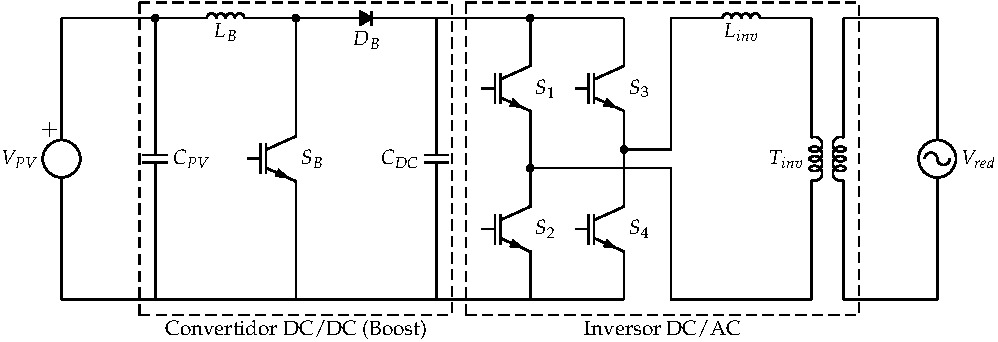
\includegraphics[width=.9\linewidth]{../figs/InversorPV.pdf}
\end{center}

\begin{itemize}
\item \alert{Filtro de entrada}: atenúa el rizado que produce la conmutación en
la corriente de entrada

\item \alert{Convertidor DC/DC}: adecúa (eleva o reduce) la tensión de salida del
generador a la tensión necesaria para el puente de conmutación. Puede
realizar las funciones de búsqueda del punto de máxima potencia.
\end{itemize}
\end{frame}

\begin{frame}[label={sec:org8871d65}]{Puente y salida}
\begin{center}
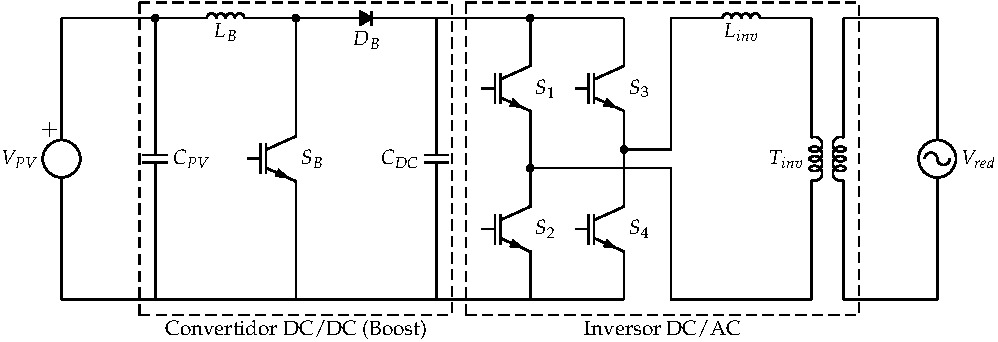
\includegraphics[width=.9\linewidth]{../figs/InversorPV.pdf}
\end{center}

\begin{itemize}
\item \alert{Puente inversor}: realiza el troceado de la señal continua para
convertirla en alterna

\item \alert{Filtro de salida}: elimina o atenúa los armónicos no deseados

\item \alert{Transformador}: adecua el valor de tensión de salida del puente al
de la red y proporciona aislamiento galvánico entre la parte DC y
AC.
\end{itemize}
\end{frame}

\begin{frame}[label={sec:orgc0d220e}]{Control}
\begin{center}
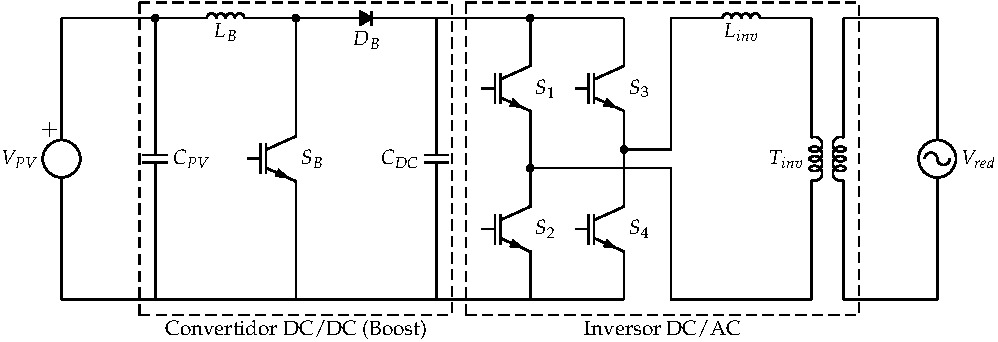
\includegraphics[width=.9\linewidth]{../figs/InversorPV.pdf}
\end{center}

\begin{itemize}
\item \alert{Control}: realiza la supervisión de la entrada y salida del
convertidor DC/DC y del puente inversor y entrega las consignas
correspondientes para localizar y seguir el MPP del generador, y para
obtener una señal sinusoidal con bajo contenido en armónicos en la
salida del inversor.
\end{itemize}
\end{frame}

\subsection{Funcionamiento}
\label{sec:orgd070f36}
\begin{frame}[label={sec:org714b432}]{Modulación SPWM}
\begin{center}
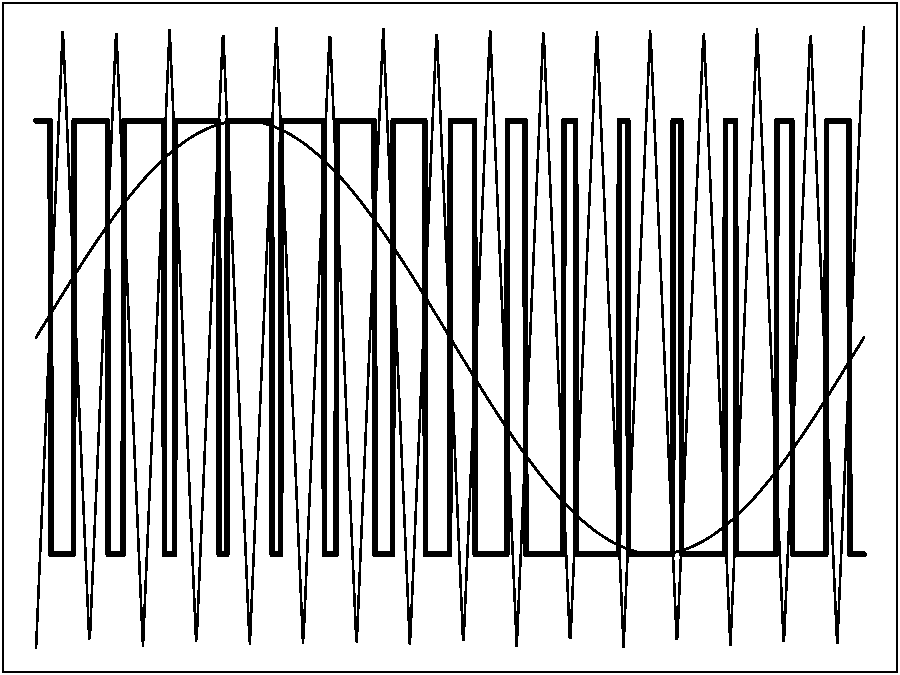
\includegraphics[width=.9\linewidth]{../figs/SPWMMonofasico.pdf}
\end{center}
\end{frame}

\begin{frame}[label={sec:org7350519}]{Busqueda del Punto de Máxima Potencia}
\begin{center}
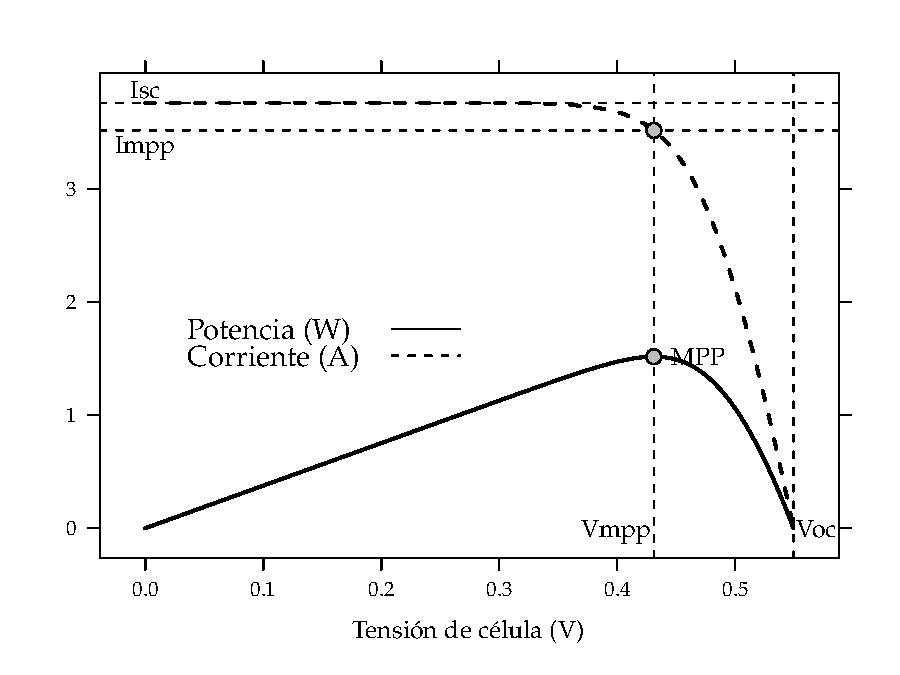
\includegraphics[height=0.6\textheight]{../figs/CurvaIV_Ta20_G800.pdf}
\end{center}

$$\begin{cases}
      \frac{dP}{dV}>0 & 0<V<V_{mpp}\\
      \frac{dP}{dV}=0 & V=V_{mpp}\\
      \frac{dP}{dV}<0 & V_{mpp}<V<V_{oc}\end{cases}$$
\end{frame}

\begin{frame}[label={sec:org723158f}]{Busqueda del Punto de Máxima Potencia}
\begin{center}
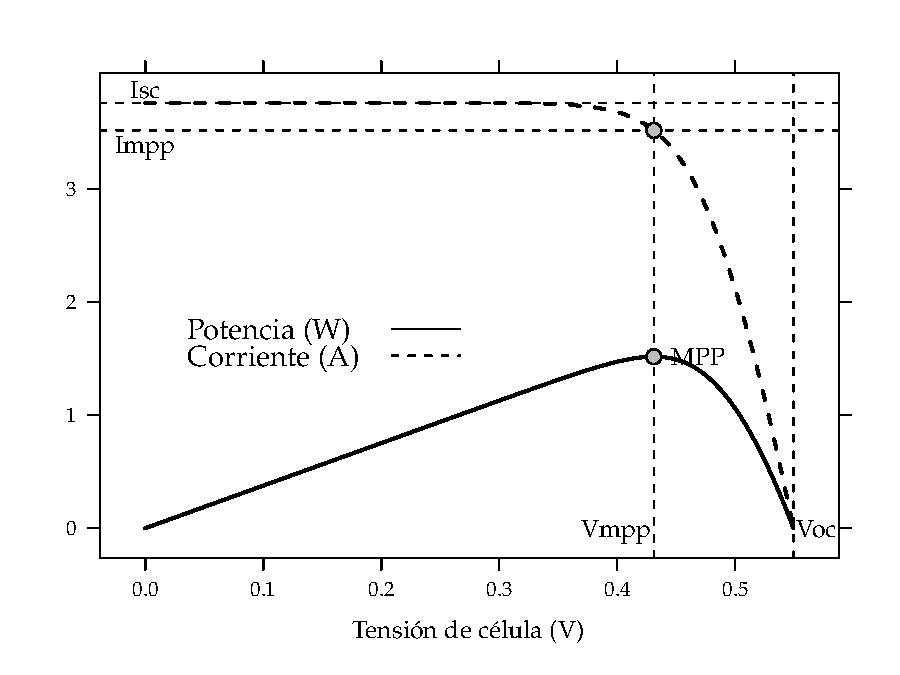
\includegraphics[height=0.6\textheight]{../figs/CurvaIV_Ta20_G800.pdf}
\end{center}

$$\begin{cases}
      \frac{dI}{dV}>-\frac{I}{V} & 0<V<V_{mpp}\\
      \frac{dI}{dV}=-\frac{I}{V} & V=V_{mpp}\\
      \frac{dI}{dV}<-\frac{I}{V} & V_{mpp}<V<V_{oc}\end{cases}$$
\end{frame}

\begin{frame}[label={sec:org669def3}]{Transformador de salida}
\begin{center}
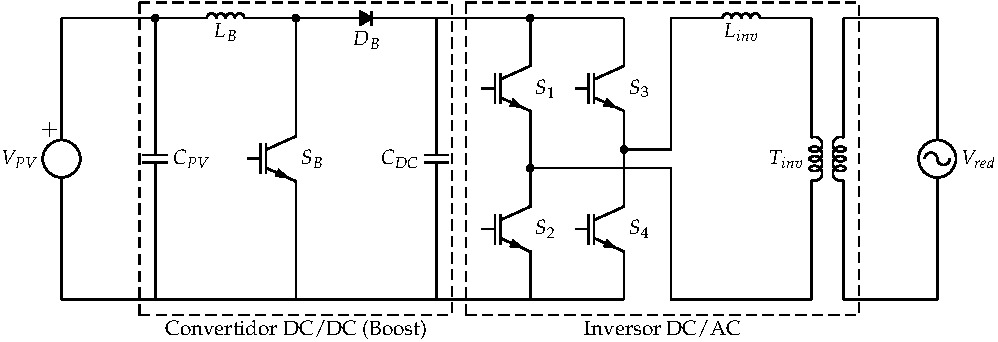
\includegraphics[width=.9\linewidth]{../figs/InversorPV.pdf}
\end{center}

\begin{itemize}
\item El transformador permite adecuar el nivel de tensión de salida del
puente de conmutación a la tensión de red.

\item La componente inductiva del transformador es parte del filtro de
salida y sirve como acoplamiento entre la red eléctrica y la salida
del inversor.

\item Establece el aislamiento galvánico entre la entrada del inversor (DC)
y la salida (AC).
\end{itemize}
\end{frame}

\begin{frame}[label={sec:org876b5a0}]{Opciones comerciales}
Existen tres opciones en el mercado de inversores de conexión a red:

\begin{itemize}
\item Inversores con transformador de salida en baja frecuencia

\item Inversores sin transformador

\item Inversores con transformador de alta frecuencia
\end{itemize}
\end{frame}

\begin{frame}[label={sec:orgfa99796}]{Normativa relativa al transformador}
La normativa vigente en España obliga al uso de un transformador de aislamiento o elemento equivalente para cumplir tres objetivos:

\begin{enumerate}
\item Aislar la instalación generadora para evitar la transferencia de defectos entre la red y la instalación

\item Proporcionar seguridad personal

\item Evitar la inyección de corriente continua en la red.
\end{enumerate}
\end{frame}

\begin{frame}[label={sec:org9c52953}]{Normativa: Nota de Interpretación Tecnica}
\begin{itemize}
\item Objetivos 1 y 2 se consiguen mediante la adecuada conexión de masas y tierras en el sistema.

\item Objetivo 3: \guillemotleft{}\alert{la corriente continua inyectada en la red de distribución por una instalación generadora no será superior al 0,5\% de la corriente nominal de la misma}\guillemotright{}, cumplido \guillemotleft{}\alert{cuando se disponga en la instalación de un transformador separador entre el inversor y el punto de conexión de la red de distribución}\guillemotright{}. \emph{Los inversores con transformador de alta frecuencia o sin transformador deben demostrar el cumplimiento de este requisito mediante un ensayo descrito en esta nota}.
\end{itemize}
\end{frame}

\subsection{Islanding}
\label{sec:orge11ffb6}
\begin{frame}[label={sec:org5836dd2}]{Definición del problema}
\begin{center}
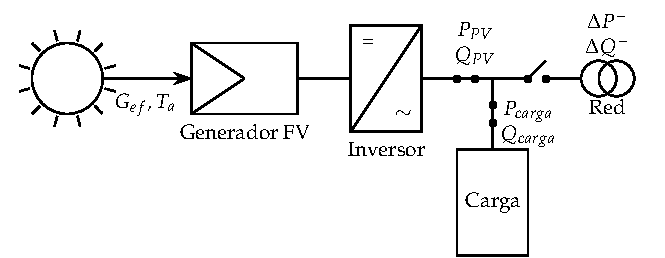
\includegraphics[width=.9\linewidth]{../figs/Isla.pdf}
\end{center}
\end{frame}

\begin{frame}[label={sec:orge5f9602}]{Ecuaciones básicas}
Antes de la desconexión:$$\Delta P=P_{carga}-P_{PV}$$

$$\Delta Q=Q_{carga}-Q_{PV}\simeq Q_{carga}$$

siendo:

$$P_{carga}=\frac{V^{2}}{R_{carga}}$$

$$Q_{carga}=\frac{V^{2}}{\omega L}-V^{2}\omega C$$
\end{frame}

\begin{frame}[label={sec:org5b83677}]{Casos posibles}
\begin{itemize}
\item \(\Delta P^{-}>0\rightarrow P_{carga}>P_{PV}\). Al producirse la
desconexión, dado que \(P_{PV}\) no cambia, disminuye la potencia
entregada a la carga, y por tanto baja la tensión.

\item \(\Delta P^{-}<0\rightarrow P_{carga}<P_{PV}\). Al producirse la
desconexión, aumenta la potencia entregada a la carga, y por tanto
sube la tensión.

\item \(\Delta Q^{-}>0\rightarrow Q_{carga}>0\). La carga es inductiva. Al
producirse la desconexión, dado que el generador FV no entrega
reactiva, la reactiva debe tender a 0, y por tanto aumenta la
frecuencia.

\item \(\Delta Q^{-}<0\rightarrow Q_{carga}<0\). La carga es capacitiva. La
reactiva debe tender a cero, y por tanto disminuye la frecuencia.
\end{itemize}
\end{frame}

\begin{frame}[label={sec:org9224e14}]{Ventana de no-detección}
Cuando las condiciones de trabajo del generador y el consumo antes de la
desconexión son muy cercanas, existe una ventana de no-detección.

\begin{center}
\begin{center}
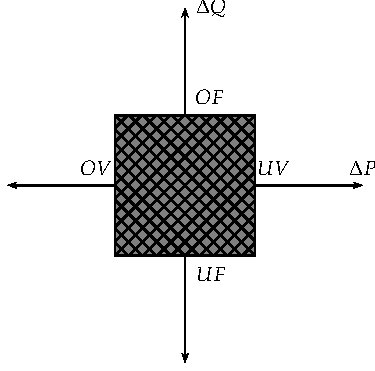
\includegraphics[height=0.6\textheight]{../figs/NDZ.pdf}
\end{center}
\end{center}
\end{frame}

\begin{frame}[label={sec:orgea0b096}]{Estudio experimental IEA-PVPS}
\begin{itemize}
\item La probabilidad de que se de una situación de balance entre consumo y
generación en una red de Baja Tensión está entre \(\num{1e-5}\) y
\(\num{1e-6}\).

\item Para que se de una situación de isla, este balance debe coincidir con
una desconexión de la red: la probabilidad de ocurrencia simultánea
de estos dos sucesos es virtualmente nula.
\end{itemize}
\end{frame}

\begin{frame}[label={sec:org5d42e58}]{Estudio experimental IEA-PVPS}
\begin{itemize}
\item El riesgo eléctrico existente en cualquier red eléctrica es del orden
de \(\num{1e-6}\).

\item Este estudio mostró que el riesgo de accidente eléctrico asociado a
un sistema fotovoltaico funcionando en isla bajo los escenarios de
mayor penetración fotovoltaica era inferior a \(\num{1e-9}\).

\item Este resultado indica que el riesgo asociado al accidente eléctrico
por isla FV no incrementa el riesgo que ya existe en las
instalaciones eléctricas.
\end{itemize}
\end{frame}
\end{document}